\section{Background}
\label{sec:background}

\subsection{Blockchain and Tangle (DAG)}
Blockchain DLT became widely known in 2009 with the launch of Bitcoin network.
Participants in the network can validate and verify the transactions independently, without relying on central trust parties.
Blockchain is usually maintained and managed by a distributed group of participants independently.
This along with its cryptographic mechanisms ensures the data recorded on the ledger immutable \cite{Yaga2018BlockchainTO}.
The structure of a traditional blockchain can be simplified as a singly linked list\footnote{Singly linked list: linked list which is unidirectional and can only be traversed in one direction.},
you can traverse from the latest block to the Genesis block\footnote{Genesis block: the first block of a blockchain. It is a special case as it does not reference a previous block.} (as shown in Fig~\ref{fig:blockchain_structure}).
Transactions are hashed in a Merkle Tree \cite{merkle1980protocols} for saving storage space and simplifying transaction validation.


\begin{figure}[h]
    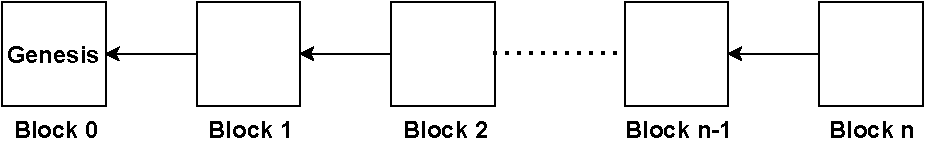
\includegraphics[width=0.45\textwidth,trim={-2cm -1cm 0 -1cm},clip]{figs/blockchain_structure.pdf}
    \caption{Blockchain structure}
    \label{fig:blockchain_structure}
\end{figure}

\begin{figure*}[t]
    \centering
    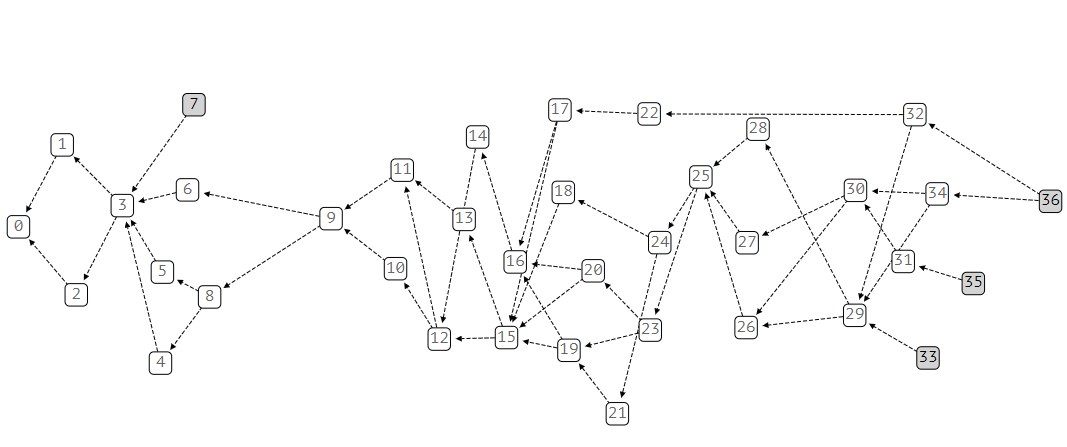
\includegraphics[width=\textwidth,trim={-1cm 0 0 2cm},clip]{figs/tangle_structure.png}
    \caption{Tangle directed-acyclic-graph structure. Shaded vertices represent tips (new transactions attaching to Tangle). The very first transaction, denoted as 0-th vertex, is the genesis transaction. It gave the total supply of IOTA tokens to one address.}
    \label{fig:tangle_structure}
\end{figure*}

In the original Bitcoin whitepaper \cite{nakamoto2008peer}, Satoshi Nakamoto has listed the procedures for handling the transactions and record them on the blockchain ledger.
All the nodes listen to the transactions broadcast to the network and each node collects new transactions for generating a new block.
Then each node will do proof-of-work and broadcast the block to the network once it finds the solution for other nodes' validation.
However, in the real case, almost all the transaction wrapping and PoW are finished by specific miners in the network. Miners also require transaction fees for the reward of doing these.
The increasing PoW complexity makes it nearly impossible to gain profit from mining Bitcoin with general PC hardware. Instead, dedicated miners have to use the equipments like ASIC\footnote{ASIC: application-specific integrated circuit. It is the integrated circuit designed for a specific use case. Bitcoin ASIC chip can only handle computing tasks for Bitcoin mining, and cannot be used for any other tasks.} specifically to the mining algorithms.
It is a potential hazard that the blockchain network will be centralized and controlled by the parties that own most of the ``mining rigs". In addition, blockchains relying on PoW are consuming massive energy \cite{sedlmeir2020energy}. According to CBECI\footnote{CBECI: Cambridge Bitcoin Electricity Consumption Index. Website: https://cbeci.org/}, Bitcoin network consumes approximately 130.51 TWh electricity per year, which is far more than the annual electricity consumption of some countries like Ukraine and Argentina. Carbon dioxide emissions caused by these PoW blockchains will cause environmental issues like global warming.


Transaction throughput and transaction confirmation latency are the two most critical performance issues about blockchain technology \cite{zhou2020solutions}.
Transactions can only be recorded on the blockchain in sequence due to its linear structure. Also, the limitation of the size of each block makes it struggling to handle the enormous volume of transactions nowadays.
Blockchains including Bitcoin and Ethereum are facing problems like low TPS and bad scalability which results in transaction backlog and high transaction fees.
To tackle these issues, people have put forward many alternative solutions such as side-chain, cross-chain, improved consensus, sharding, DAG, etc.
IOTA Tangle is a new type of DLT addressing solving the problems above for IoT services. It has the following advantages comparing with traditional blockchain technologies:

\begin{enumerate}
    \item \textbf{High scalability.} Directed-acyclic-graph structured Tangle ledger enables its high scalability. Serguei Popov has analyzed the performances of the system under two different regimes: low load and high load in the article \textit{The Tangle} \cite{popov2015tangle} In high load regime when more new tips\footnote{Tip: every new (unconfirmed) transaction is known as a tip.} are attached to Tangle, the typical time of a tip being approved is reduced.
          So the larger the scale of the network, the more efficient it will be.
    \item \textbf{Feeless \& Environmentally Friendly.} In a DLT network like Bitcoin, we need to pay transaction fees to the miners for rewarding them wrapping our transactions to the block and conducting PoW computations. Transaction fees are considered part of the incentive for nodes to support the network. In IOTA Tangle, however, PoW consensus and miners are removed \cite{popov2019iota}. So it is more economical and environmentally Friendly to use Tangle for sending transactions.
    \item \textbf{Quantum Robust Cryptography.} IOTA Tangle uses post-quantum cryptography for securing data on the ledger \cite{tennant2017improving}. For instance, IOTA uses Winternitz One-Time Signature (WOTS), which is promising to be resistant to quantum computers \cite{buchmann2008post} as a signature scheme protocol.
    \item \textbf{Lightweight.} IOTA node applications like GoHornet\footnote{GoHornet: IOTA full node software built in Go. Github source code: https://github.com/gohornet/hornet} is lightweight and can be easily installed and run on low-end devices such as Raspberry Pi 4.
\end{enumerate}

These characteristics are very crucial for IoT applications and favorable for critical data binding and sharing of Vivian.


\subsection{Decentralized Naming System}
Before distributed ledger technology came into being, building a decentralized naming system was considered almost impossible \cite{swartz_2011}. To build a system like it, three properties have to be satisfied:

\begin{enumerate}
    \item \textbf{Human-meaningful.} The names the system provides should be meaningful and easy to memorize, e.g. bitcoin.org. And hash values like \texttt{764569e58f53} are obviously not meaningful and hard for people to memorize.
    \item \textbf{Secure.} The names should return the correct binding values. Damage caused by malicious entities should be as low  as possible.
    \item \textbf{Decentralized.} No central authority controls the system. Names can be chosen by users at the edge of the network rather than representative central parties.
\end{enumerate}

The challenge is that, with traditional approaches, a naming system can satisfy some of the properties, but not all three of them at the same time \cite{wilcox2001names}. This trilemma is called Zooko's triangle \cite{swartz_2011} (very similar to CAP theorem\footnote{CAP theorem: it is impossible for a distributed data store to provide, Consistency, Availability and Partition tolerance, all of the three guarantees simultaneously.} in distributed system design).
Besides, the system should also ensure the uniqueness of the names, which means two different users cannot create and use the same name \cite{ali2017blockstack}.
Domain Name System in the current Internet is human-meaningful and secure, but not decentralized. Public keys are secure and decentralized, but not human-meaningful.
Zooko's Triangle has been squared by distributed ledger technology \cite{swartz_2011} and Namecoin was the first implementation to build a decentralized naming system over blockchain DL.

\begin{figure}[h]
    \centering
    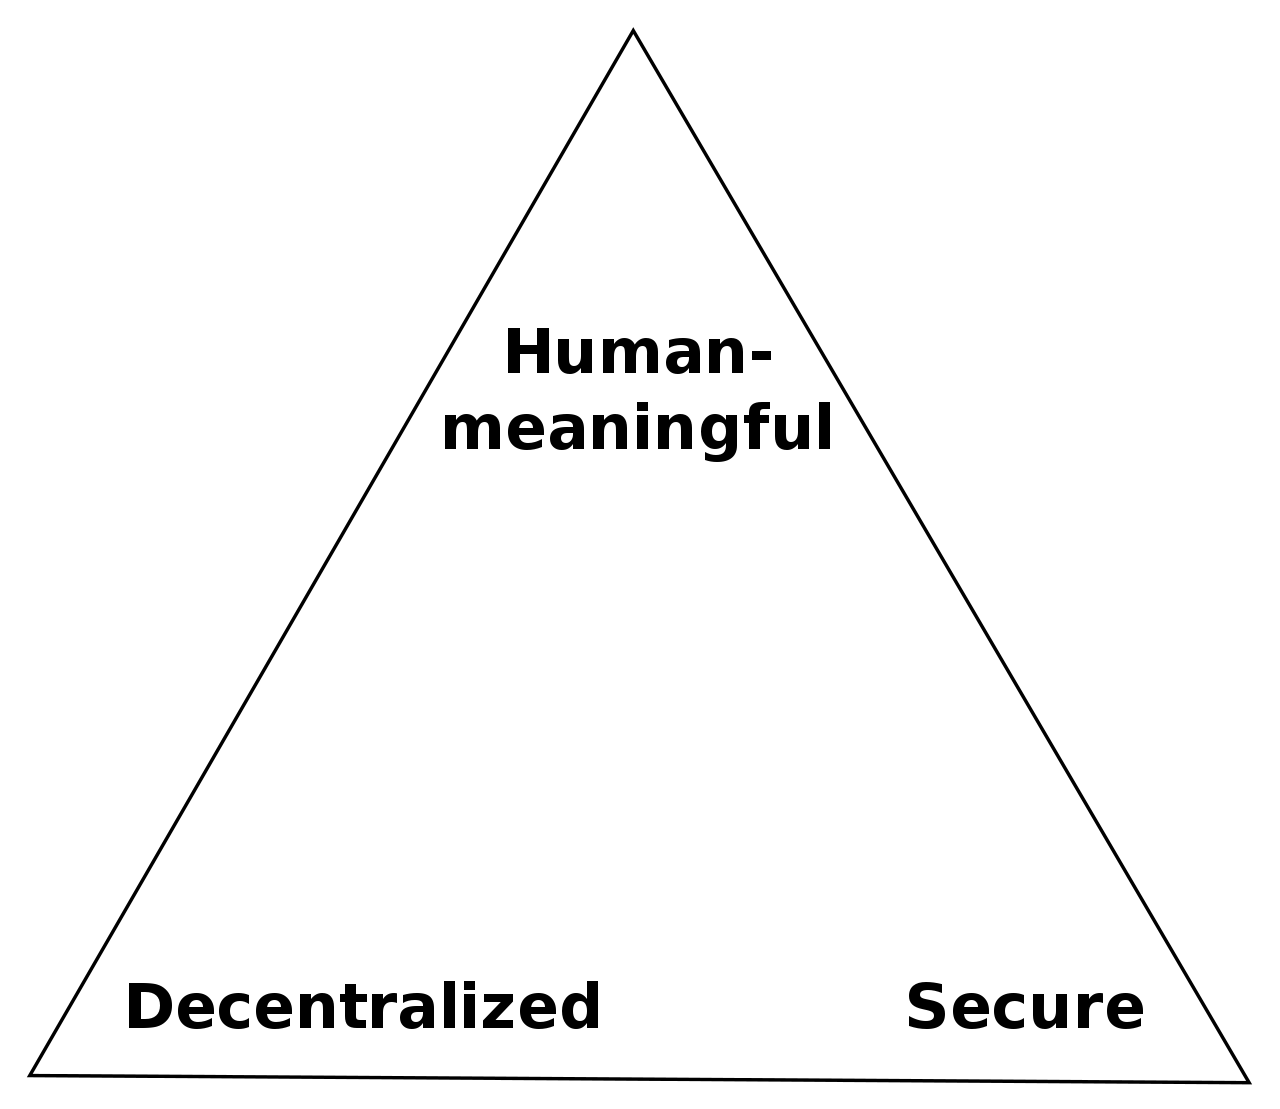
\includegraphics[width=0.2\textwidth,trim={0 0 0 0},clip]{figs/zooko_triangle.png}
    \caption{Zooko's Triangle}
    \label{fig:zooko_triangle}
\end{figure}

Blockstack is a decentralized public key infrastructure (PKI) service built on Bitcoin for building a decentralized Internet \cite{ali2017blockstack}.
The implementation of its naming system is based on the definition of a state machine and rules for state transitions on its virtualchains \cite{nelson2016extending, ali2016blockstack}.
In the design of Vivian's naming system, we referenced the ideas from Blockstack and Namecoin.

\subsection{P2P Network}

In conclusion, peer-to-peer (P2P) networks are distributed networks in which participants provide service and content that can be accessed by other peers directly without passing through intermediate entities by shared hardware resources \cite{990434}.
In a P2P network, all the peers are equally privileged, equipotent nodes that forming the network \cite{nemat2011taking}. Unlike the client-server model, a peer plays the roles of suppliers and consumers of the sources at the same time.

\subsubsection{Peer Discovery}
In a P2P network, resources like shared files are stored on different servers in a distributed way.
In normal client-server model, if a client wants to find another node or specific resources in the network, it usually sends requests to the central servers for targets' information.
In the original implementation in BitTorrent \cite{bram_2008}, a well-known P2P file sharing protocol, tracker servers keep the global registry of all the downloaders and seeds of the corresponding files \cite{pouwelse2005bittorrent}.
When the trackers are crashed or taken down, peers will not be able to connect with other peers and retrieve the files successfully. Later on a decentralized approach for finding other peers has been come up with: Distributed Hash Table (DHT).
In Vivian, we use \textbf{Kademlia Distributed Hash Table (Kad-DHT)} \cite{maymounkov2002kademlia} for peer discovery. In Kademlia, DHT is used for storing the resources location in the network. Every node and key has a unique ID (usually 160 bits).
And each value is stored at the nodes whose ID are closest to the key ID. The distance between every two nodes are calculated as exclusive or (XOR) of the two nodes' IDs.
When searching through n nodes in the system, Kad-DHT only needs to contact $O\log (n)$ nodes.

\begin{figure}[h]
    \centering
    \begin{subfigure}[t]{0.45\textwidth}
        \centering
        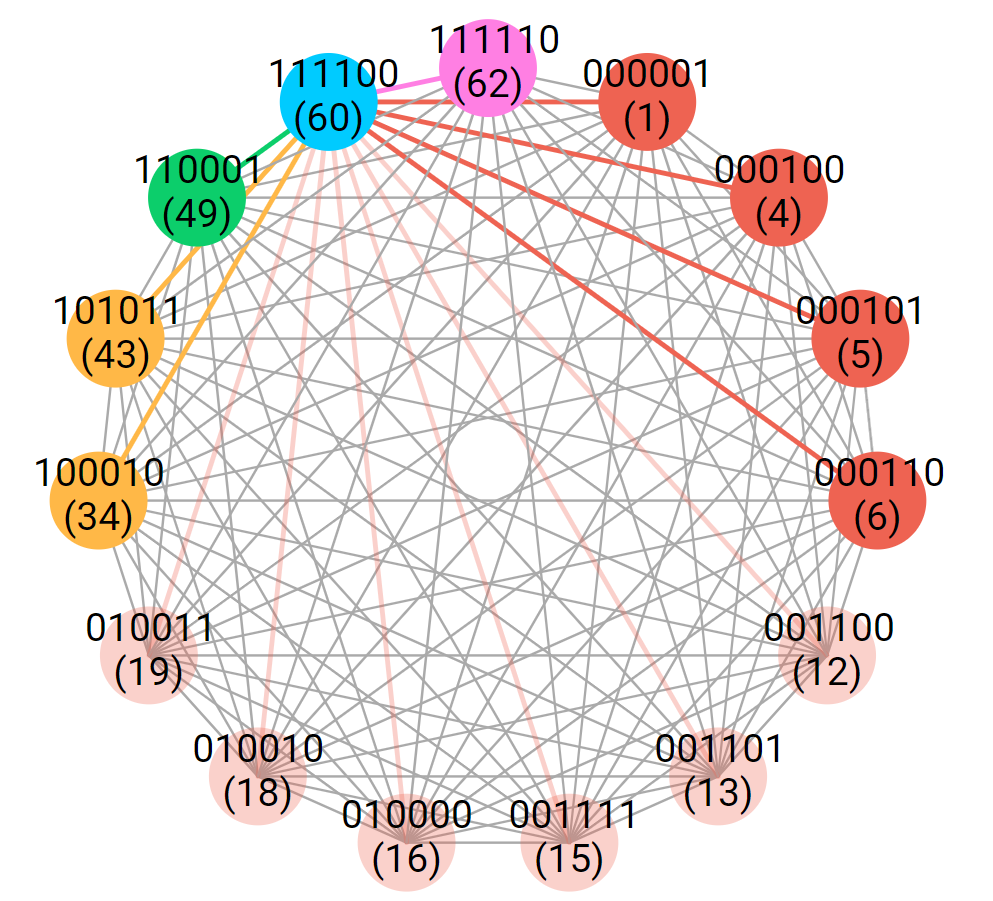
\includegraphics[width=0.7\textwidth,trim={0 0 0 0},clip]{figs/kad_k_bucket.png}
        \centering
        \caption{All nodes}
    \end{subfigure}
    \centering
    \begin{subfigure}[b]{0.45\textwidth}
        \centering
        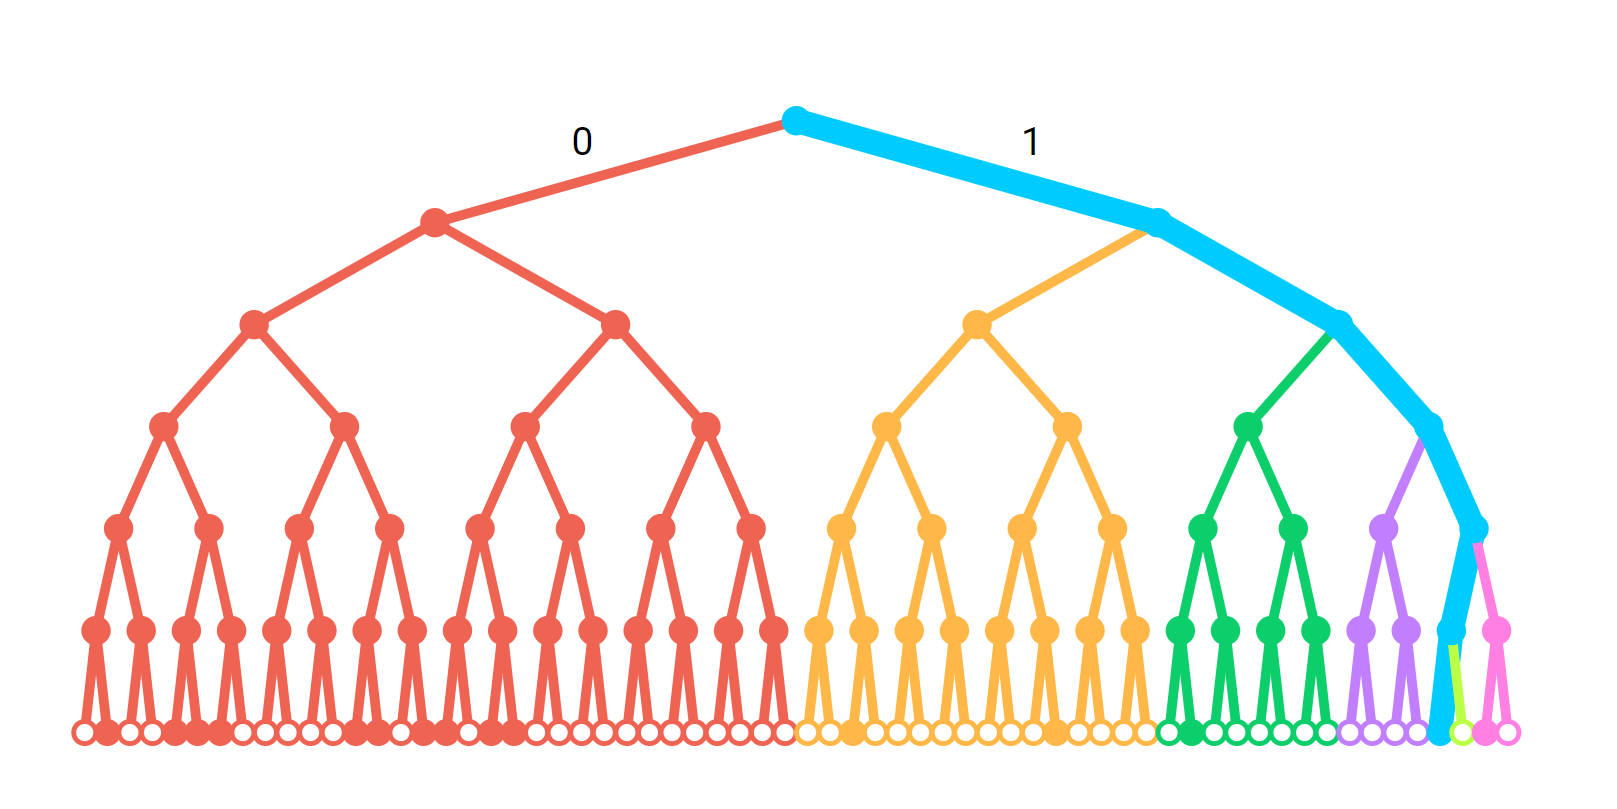
\includegraphics[width=0.9\textwidth,trim={0 0 0 -3.0cm},clip]{figs/kad_binary_tree.png}
        \centering
        \caption{Binary tree based on node ID}
    \end{subfigure}
    \caption{Kademlia DHT. In this example, node ID is 6 bits, and routing table size is 64. Originating the look-up at Node 60 (111100), the k-buckets for it is [(1, 4, 5, 6), (34, 43), (49)] when k = 4 and alpha = 3.}
    \label{fig:kad_dht}
\end{figure}

Another peer discovery method used in Vivian is \textbf{Multicast DNS (mDNS)} \cite{cheshire2013multicast}. In mDNS protocol, a device in the local area network broadcasts message to all the other devices in the network to tell them its identity and address. The other devices which enable mDNS will respond corresponding message after receiving the broadcast message.

\subsubsection{Peer Communication}

Nodes in Vivian use \textbf{Gossip Protocol} \cite{10.1145/41840.41841} for dissemination of information such as naming key-value bindings. It is a eventual consistency algorithm based on the way of epidemic spreads.
Gossip protocol has advantages like simple, highly scalable, faut-tolerant, and decentralized. Many platforms such as Redis Cluster, Consul, Apache Cassandra, and Bitcoin are using this protocol.